\chapter{Background} \label{ch:background}

This chapter presents the foundational concepts that support the methods and systems used in this thesis. This thesis is at the intersection of robotics, simulation, reinforcement learning, and neuro-symbolic AI. Each of these areas is described below in the context of this work to provide background on the development of the robotic test platform and proposed neuro-symbolic model.

\section{Robotic Manipulators} \label{se:robotic_manipulators}
Robotic manipulators are commonly used in industrial and research applications due to their precision and versatility. These systems typically consist of multiple joints (degrees of freedom) that allow an end effector to move and manipulate objects in 3D space. This thesis focuses on a 6-axis robotic manipulator, capable of performing complex tasks such as grasping, moving, and orienting objects. The flexibility of these robots makes them ideal for testing reinforcement learning algorithms, especially in multi-task settings.

\subsection{6-Axis Robotic Manipulators} \label{ss:6axis}
Six-axis arms offer a rich action space and are commonly used in industrial automation. Their joints—usually revolute—enable motion in three-dimensional space, with pitch, yaw, and roll control over the end effector. These properties make them suitable for fine-grained motion planning and manipulation tasks, especially when paired with a learning-based controller.

\section{Control Software \& Simulation} \label{se:simulation}
To safely develop and test control algorithms, robotic systems are often simulated before being deployed in real-world settings. This thesis leverages the Robot Operating System (ROS2) middleware and the Gazebo Harmonic physics simulator to create a modular, testable robotic platform.

\subsection{Robot Operating System (ROS2)} \label{ss:ros2}
ROS2 is a widely adopted middleware framework that supports distributed communication, modular design, and hardware abstraction for robotic systems. It allows for flexible integration between control algorithms, sensors, and actuators, making it an ideal tool for reinforcement learning research.

\subsection{Gazebo Simulation Environment} \label{ss:simulation}
Gazebo provides realistic physics-based simulation of robots and their environments. It supports a variety of sensors, actuators, and physics engines, making it a powerful tool for testing learning-based control in a safe and controlled environment. In this work, Gazebo Harmonic is used to simulate the physical properties of the 6-axis robot and its interaction with objects.

% \section{Markov Decision Process} \label{se:markov_decision_process}
\section{Reinforcement Learning} \label{se:reinforcement_learning}
Reinforcement Learning (RL) is a paradigm where agents learn to make decisions by interacting with an environment. At each timestep, an agent observes a state, performs an action, and receives a reward based on the outcome. Over time, the agent learns a policy that maximizes cumulative reward.

\subsection{Deep Reinforcement Learning} \label{ss:deep_reinforcement_learning}
Deep RL leverages deep neural networks to approximate policies or value functions in high-dimensional state spaces. It allows agents to learn directly from raw inputs like images or sensor data. Algorithms like DQN and PPO have been successful in a variety of domains, but often lack interpretability.

\subsection{Deep Deterministic Policy Gradient} \label{ss:deep_deterministic_policy_gradient}
DDPG is an off-policy actor-critic algorithm designed for continuous action spaces. It combines value-based and policy-based methods by training a deterministic policy alongside a Q-function. In this work, DDPG is used as the primary reinforcement learning method for robotic control tasks.

\subsection{Hindsight Experience Replay} \label{ss:hindsight_experience_replay}
HER enhances sample efficiency in sparse reward environments by relabeling failed experiences as successful ones based on alternative goals. This allows agents to learn from episodes that would otherwise provide little learning signal. HER is particularly useful in goal-conditioned tasks such as pick-and-place.

\section{Neuro-symbolic AI} \label{se:neurosymbolic_ai}

\begin{figure}[htb]
	\centering
	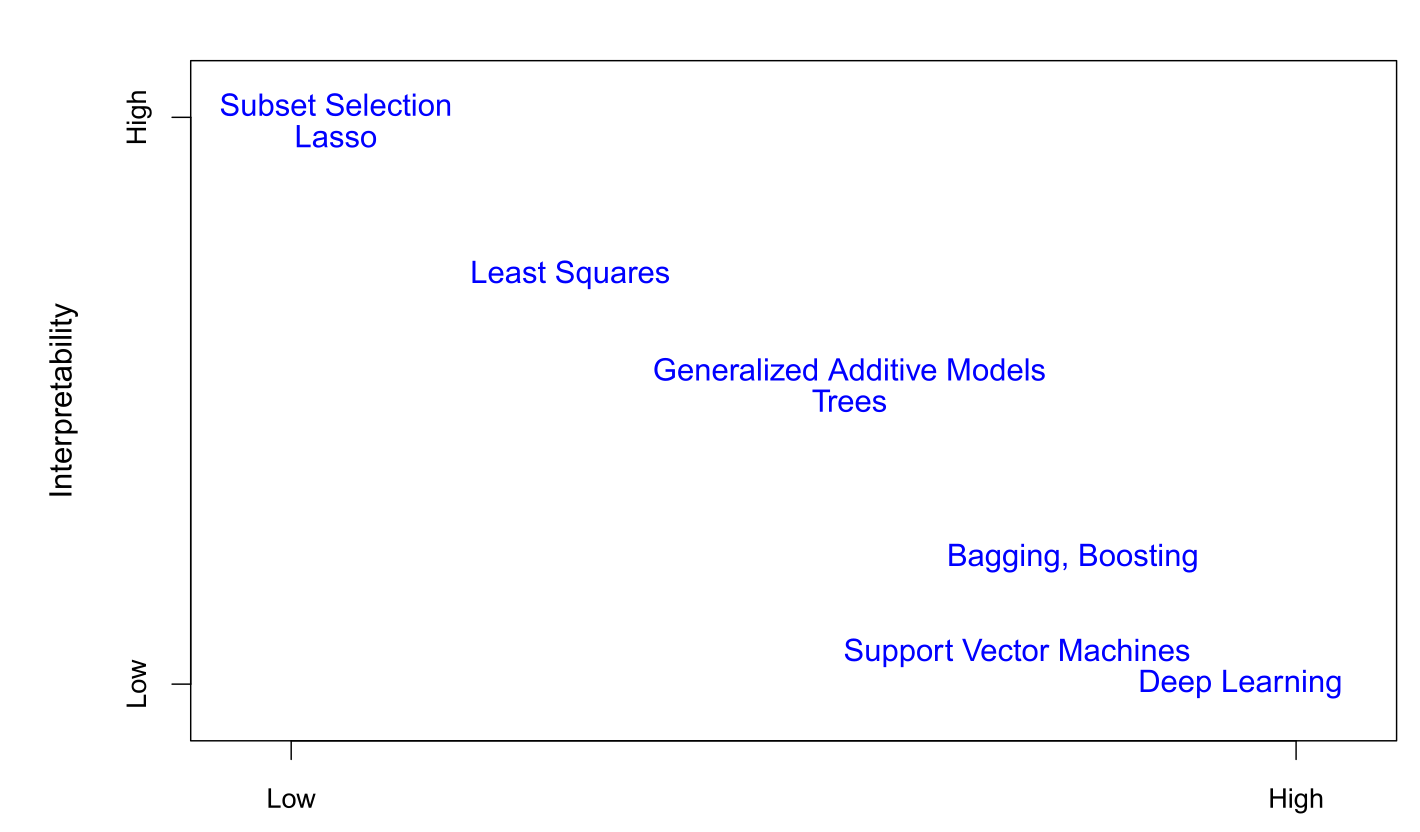
\includegraphics[scale=0.25]{./images/interpretability_vs_flexibility.png}
	\caption{Trade-off between interpretabilty and model flexibility} 
\end{figure}

Neuro-symbolic models can be broadly defined as models which focus on merging both \textit{neural} and \textit{symbolic} AI approaches to add value to the system. The term \textit{nerual} refers to the use of artificial neural networks and the term \textit{symbolic} typically refers to approaches based on explicit symbol manipulation. (CITATION taxonomy.pdf) The fundamental desire of neuro-symbolic models is to leverage both neural and symbolic approaches in a way that is favorable to the strengths of each approach and unfavorable to their weaknesses. The strengths neural models would include the ability to leverage raw data that may be too dificult/complex to semantically reason about, while the weaknesses may include the challenges faced when attempting to reason neural models. Conversely, the strengths of symbolic models include their ability to be highly explainable and verifiable, but they may have weaknesses in their reliance human input/understanding of a system. Thus, the promise of a neuro-symbolic architecture is a system which would be robust from training data, symbolically explainable, and be able to leverage human expert knowledge in its design. 

In recent years many different neuro-symbolic models have been designed and deployed. Because the intersection of these two approaches may be quite broad and models can take many different forms be it is important to make distinctions between the various incarnations of neuro-symbolic architectures. Henry Kautz, in a 2005 article presents "six possible designs" patterns classifying each method in reference to their neural and symbolic interactions:(CITATION KAUTZ)

\subsection{Classification of Neuro-symbolic Architectures} \label{ss:classification}
\begin{scriptsize}
	\begin{center}
		\begin{tabular}{ | m{5cm} | m{5cm}| m{5cm} | }
			\hline
			\textbf{Neuro-symbolic Design Pattern} & \textbf{Definition} & \textbf{Example}\\
			\hline
			Symbolic Neural symbolic & A symbolic input is fed into a neural network producing a symbolc output. & GPT \\
			\hline
			Symbolic[Neural] & A neural subroutine is evoked by a symbolic strategy. & AlphaGo \\
			\hline
			Neural[Symbolic] & A symbolic subroutine is evoked by a neural strategy. & ChatGPT accessing Wolfram for computations\\
			\hline
			Neural|Symbolic & A neural network converts a non-symbolic input into symbolic data to be symbolically processed. & Neuro-Symbolic Concept Learner \\
			\hline
			Neural:Symbolic $\rightarrow$ Neural & A symbolically represented dataset is used to train an neural network to predict a symbolic output & ANN-MPC \\
			\hline
			Neural\_\{Symbolic\} & Symbolic rules are used to define the structures making up the neural network. & Logic Tensor Networks \\
			\hline
		\end{tabular}
	\end{center}
\end{scriptsize}
\subsection{Neuro-symbolic Concept Learner} \label{ss:neurosymbolic_concept_learner}
The Neuro-Symbolic Concept Learner (NS-CL), developed by Mao et al., is a representative example of the Neural|Symbolic pattern. It combines convolutional and recurrent networks to extract structured representations from images and language, which are then processed by a symbolic reasoning module. This thesis adapts NS-CL to preprocess environment observations and task instructions for reinforcement learning.

\section{Neuro-symbolic Reinforcement Learning} \label{se:neurosymbolic_rl}
Neuro-symbolic reinforcement learning (NSRL) is an emerging field that merges symbolic abstraction with RL policies. The aim is to produce agents that can learn effectively from data while providing semantic interpretability. NSRL allows for modular design, generalization across tasks, and the integration of external knowledge sources (e.g., task graphs or logic rules). In this thesis, NSRL is explored through a novel adaptation of NS-CL to guide robotic agents using natural language prompts and symbolic scene representations.

% \section{Sim-to-Real} \label{se:sim_to_real}
% \subsection{Transfer Learning} \label{ss: transfer_learning}
% \subsection{Multitask Learning} \label{ss:multitask_learning}
